\chapter{Results}
\label{chapter:results}

\section{Basic setup}
In this section we trained the model with the parameters described in chapter \ref{chapter:methods}.
\subsection{YOLOv5}
The results of the YOLOv5 model for training and test dataset are available in table \ref{tab:yolov5_basic}, and more in-depth information about the $AP$ can be seen from precision-recall curves for which are plotted in figure \ref{fig:yolov5_pr_curves}. Furthermore, samples from the test part of the dataset with overlayed predictions and ground truth boxes are in the appendix \ref{appendix:model_predictions}.
\begin{table}
    \begin{tabular}{c|c|c|c|c|c|c|c}
        stage & $AP$  & $AP@.3$ & $AP@.5$ & $AP@.75$ & $AP@.5_S$ & $AP@.5_M$ & $AP@.5_L$ \\ \hline
        train & 0.463 & 0.869   & 0.841   & 0.442    & 0.697     & 0.887     & 0.974     \\ \hline
        test  & 0.249 & 0.734   & 0.631   & 0.132    & 0.598     & 0.671     & 0.607     \\
    \end{tabular}
    \caption{Mean average precision of the YOLOv5 model}
    \label{tab:yolov5_basic}
\end{table}

\begin{paracol}{2}
    \begin{figure}
        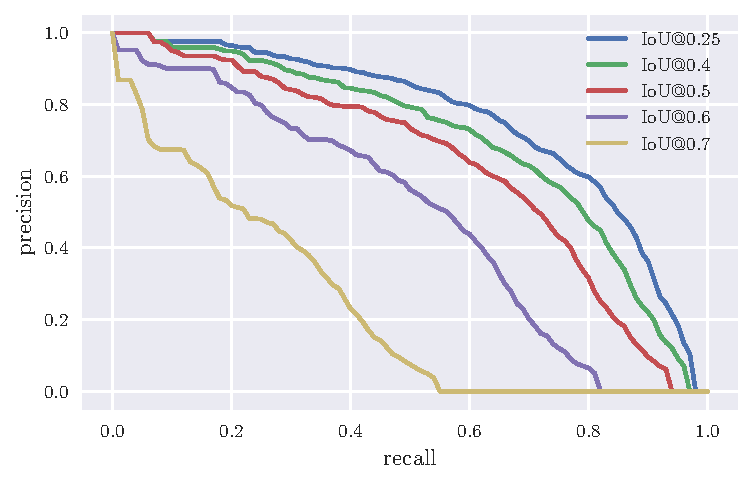
\includegraphics[width=\linewidth]{images/iou_val_multiple.pdf}
        \caption{Precision-recall curve of the YOLOv5 model}
        \label{fig:yolov5_pr_curves}
    \end{figure}
    \switchcolumn
    \begin{figure}
        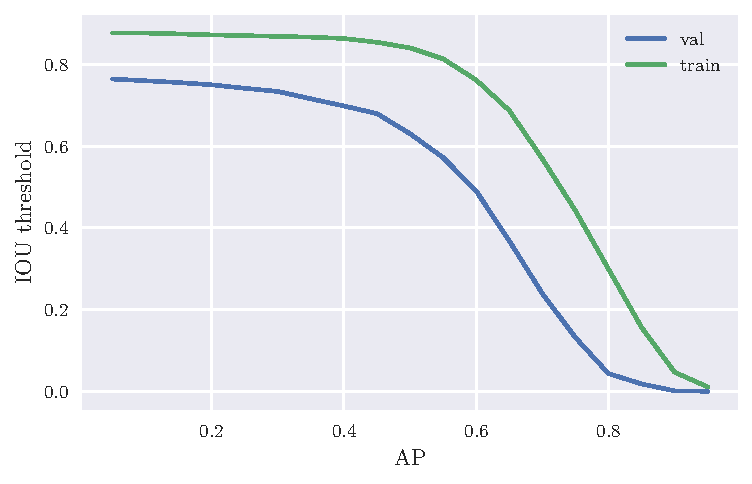
\includegraphics[width=\linewidth]{images/iou_threshold.pdf}
        \caption{The value of MAP based on the IOU threshold $\gamma$}
        \label{fig:yolov5_map_iou_thresholds}
    \end{figure}
\end{paracol}

\subsection{EfficientDet}
We evaluated the EfficientDet model in the same fashion as YOLOv5 and resulting metrics are strored into the table \ref{tab:effdet_basic}.
\begin{table}
    \begin{tabular}{c|c|c|c|c|c|c|c}
        stage      & $AP$  & $AP@.3$ & $AP@.5$ & $AP@.75$ & $AP@.5_S$ & $AP@.5_M$ & $AP@.5_L$ \\ \hline
        training   & 0.297 & 0.82    & 0.735   & 0.164    & 0.552     & 0.838     & 0.815     \\ \hline
        validation & 0.168 & 0.666   & 0.525   & 0.041    & 0.435     & 0.606     & 0.527     \\
    \end{tabular}
    \caption{Mean average precision of the EfficientDet model}
    \label{tab:effdet_basic}
\end{table}


\section{Experiments}
The YOLOv5 model was selected since it was better performing than EfficientDet. Unless stated otherwise, we kept the same parameters as described in chapter\ref{chapter:methods}. Through a series of experiments, we tried to get an insight into the importance of model parameters.
\subsection{Different backbones}
We changed the batch size to 2 (to fit 5x6 backbone into the GPU memory) and trained the model with different backbones for 50 epochs each. Results of all runs are in table \ref{tab:yolov5_backbones}.

\begin{table}
    \begin{tabular}{c|c|c|c|c|c}
        Backbone & $AP@.5$ & $AP$  & Parameters[M] & Flops[G] & Time[h] \\ \hline
        5s6      & 0.593   & 0.231 & 12            & 21       & 2.1     \\ \hline
        5m6      & 0.621   & 0.242 & 35            & 63       & 3.5     \\ \hline
        5l6      & 0.611   & 0.241 & 76            & 141      & 5.2     \\ \hline
        5x6      & 0.601   & 0.238 & 140           & 267      & 8.5     \\
    \end{tabular}
    \caption{Results of the YOLOv5 architecture with different backbones}
    \label{tab:yolov5_backbones}
\end{table}

\subsection{Different image size}
Once again, we kept the same setting and changed only the size to which images are resized. The relation between input image size and $AP@.5$ can be observed in figure \ref{fig:img_sizes}.

\begin{paracol}{2}
    \begin{figure}
        \centering
        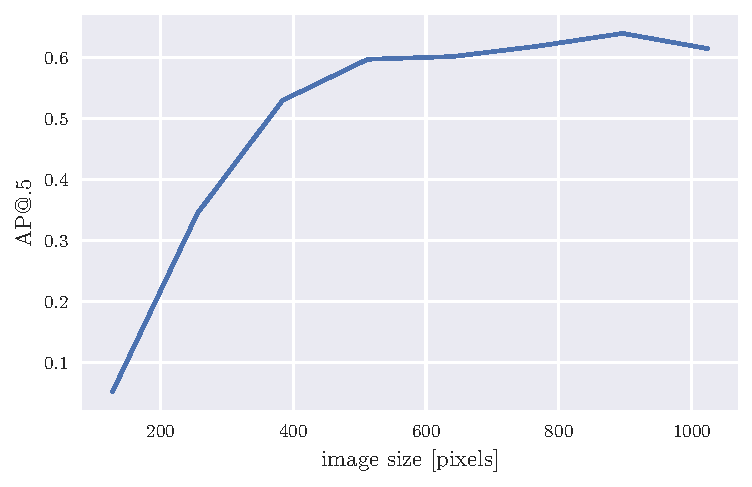
\includegraphics[width=0.99\linewidth]{images/img_size_dependency.pdf}
        \caption{The relation between image size and $AP@.5$}
        \label{fig:img_sizes}
    \end{figure}
    \switchcolumn
    \begin{figure}
        \centering
        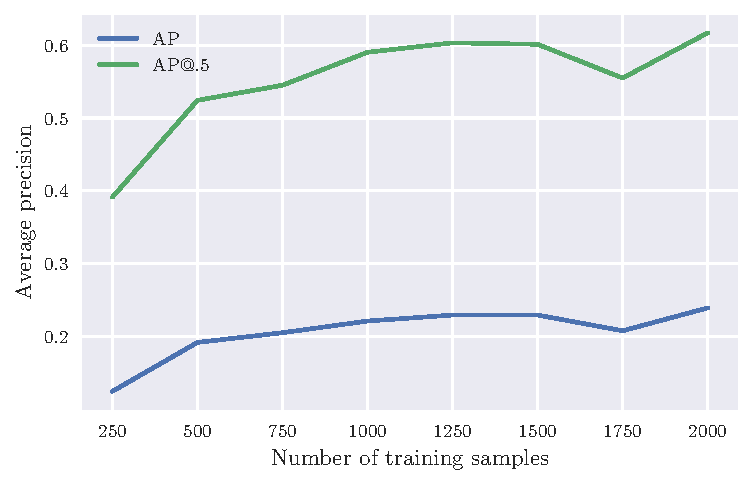
\includegraphics[width=0.99\linewidth]{images/training_set_dependency.pdf}
        \caption{Mean average precision based on the size of training set}
        \label{fig:training_set_sizes}
    \end{figure}
\end{paracol}

% \begin{figure}
%     \begin{minipage}{0.49\textwidth}
%         \centering
%         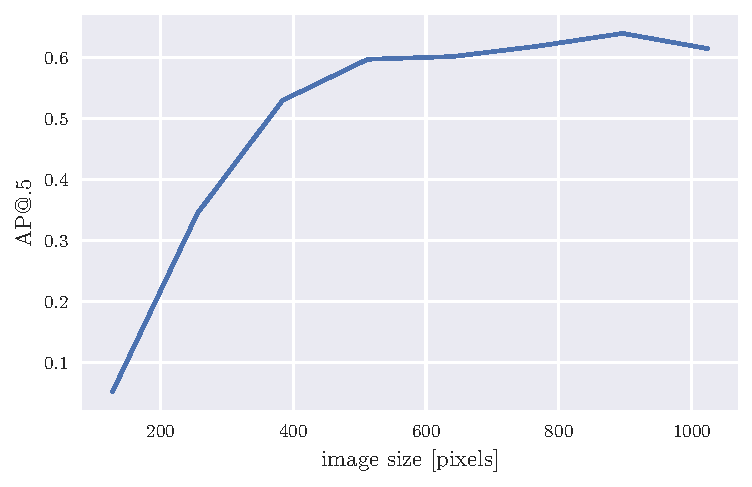
\includegraphics[width=0.99\linewidth]{images/img_size_dependency.pdf}
%         \caption{The relation between image size and $AP@.5$}
%         \label{fig:img_sizes}
%     \end{minipage}
%     \begin{minipage}{0.5\textwidth}
%         \centering
%         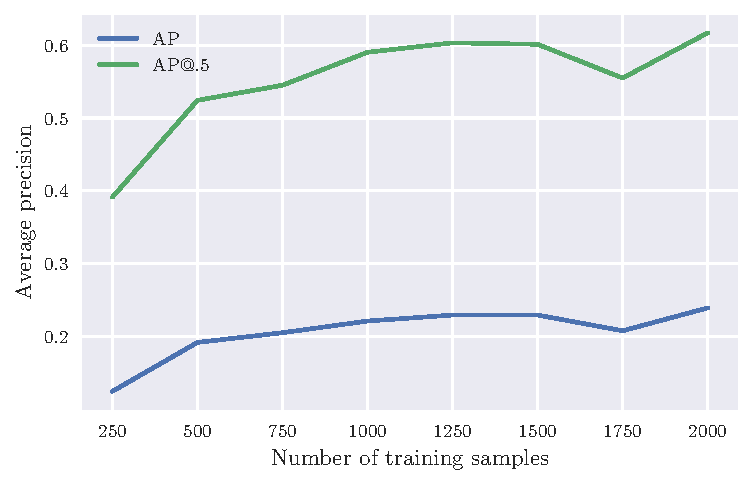
\includegraphics[width=0.99\linewidth]{images/training_set_dependency.pdf}
%         % \caption{Mean average precision based on the size of training set}
%         \caption{Mean average precision based on the size of training set}
%         \label{fig:training_set_sizes}
%     \end{minipage}
% \end{figure}
\begin{figure}
    \begin{floatrow}[2]
        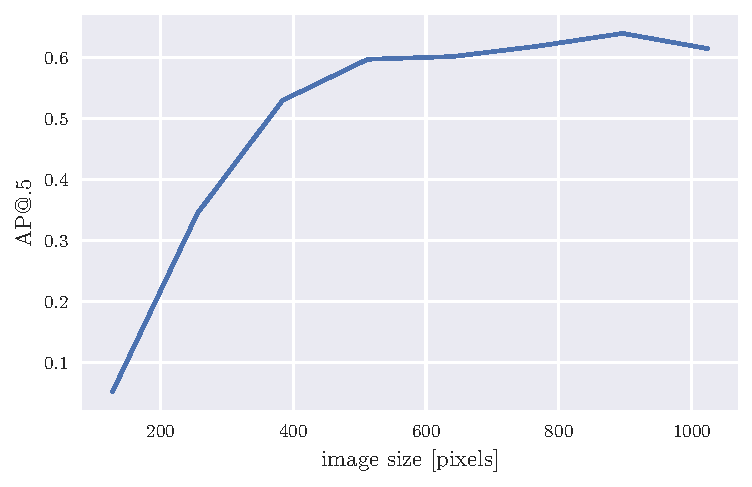
\includegraphics[width=0.5\linewidth]{images/img_size_dependency.pdf}\qquad
        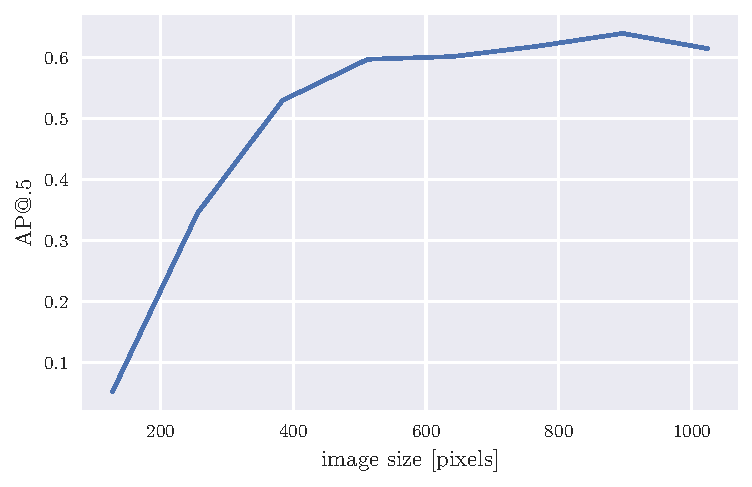
\includegraphics[width=0.5\linewidth]{images/img_size_dependency.pdf}\qquad
    \end{floatrow}
\end{figure}

\section{Ensembling}
\subsection{Grid search results}

% \subsection{Reduced training dataset}
% We fixed the validation and test dataset and changed the number of samples in the training dataset. The dependency of $AP$ on the number of training samples is depicted in figure \ref{fig:training_set_sizes}.


\begin{table}
    \begin{tabular}{c||c|c|c|c|c|c}
        Method & FRCNN-R50      & YOLOV5-M       & RET-SWINT      & FRCNN-R101     & $T$  & $\sigma$ \\ \hline
        nms    & 1              & 0.4            & 0.4            & 0.85           & 0.6  &          \\ \hline
        snms   & 1              & 0.12           & 0.12           & 0.12           & 0.7  & 0.8      \\ \hline
        nwm    & 0.85           & 0.25           & 0.70           & 0.85           & 0.45 &          \\ \hline
        wbf    & 1              & 0.4            & 0.85           & 0.85           & 0.65 &          \\ \hline
        wbf-A  & 0.94/0.77/0.84 & 0.31/0.47/0.31 & 0.98/0.85/0.88 & 0.72/0.69/0.91 & 0.64 &          \\ \hline
    \end{tabular}
    \caption{}
\end{table}


\begin{table}
    \centering
    \begin{tabular}{c|c|c|c|c|c|c|c}

        method & $AP$  & $AP@.3$ & $AP@.5$ & $AP@.75$ & $AP@.5_S$ & $AP@.5_M$ & $AP@.5_L$ \\ \hline \hline
        nms    & 0.346 & 0.818   & 0.735   & 0.28     & 0.618     & 0.775     & 0.829     \\ \hline
        snms   & 0.348 & 0.807   & 0.722   & 0.295    & 0.609     & 0.758     & 0.819     \\ \hline
        nwm    & 0.364 & 0.829   & 0.759   & 0.302    & 0.641     & 0.802     & 0.854     \\ \hline
        wbf    & 0.378 & 0.832   & 0.77    & 0.323    & 0.663     & 0.807     & 0.875     \\ \hline
        wbf-A  & 0.376 & 0.832   & 0.768   & 0.318    & 0.651     & 0.806     & 0.875     \\ \hline
    \end{tabular}
\end{table}


\begin{table}
    \centering
    \begin{tabular}{c|c|c|c|c|c|c|c}
        enms  & 0.546 & 0.91  & 0.971 & 0.522 & 0.949 & 0.98  & 0.98  \\ \hline
        snms  & 0.584 & 0.888 & 0.951 & 0.603 & 0.912 & 0.965 & 0.965 \\ \hline
        nwm   & 0.526 & 0.913 & 0.941 & 0.513 & 0.892 & 0.959 & 0.959 \\ \hline
        wbf   & 0.573 & 0.918 & 0.975 & 0.569 & 0.956 & 0.981 & 0.981 \\ \hline
        wbf-A & 0.572 & 0.92  & 0.974 & 0.566 & 0.956 & 0.98  & 0.98  \\ \hline
    \end{tabular}
\end{table}


\begin{table}
    \begin{tabular}{c||c|c|c|c}
        Model - backbone & Precision & Recall & F-score & Confidence threshold \\ \hline \hline
        nms              & 0.708     & 0.68   & 0.694   & 0.284                \\ \hline
        snms             & 0.679     & 0.7    & 0.689   & 0.489                \\ \hline
        nwm              & 0.713     & 0.71   & 0.712   & 0.792                \\ \hline
        wbf              & 0.732     & 0.7    & 0.715   & 0.594                \\ \hline
        wbf-A            & 0.745     & 0.69   & 0.716   & 0.201                \\ \hline
    \end{tabular}
    \caption{Precision, recall, and F-score based on the confidence threshold for different ensembling methods}
    \label{tab:ensembling_prf}
\end{table}
